\subsection{Quick Sort}

\subsubsection{Core concept}
Quick sort is a sorting algorithm based on the Divide and Conquer algorithm that picks an element as a pivot and partitions the given array around the picked pivot by placing the pivot in its correct position in the sorted array. It one of best sorting algorithms using key comparisons. 

\subsubsection{Explanation}

The algorithm consists of the following three steps: ~\cite{ref1}
\begin{itemize}[label=-]
    \item Divide: Partition the list.
    \begin{itemize}[label=$\bullet$]
        \item To partition the list, we first choose some element from the list for which we hope about half the elements will come before and half after. Call this element the pivot.
        \item Then we partition the elements so that all those with values less than the pivot come in one sub-list and all those with greater values come in another.
    \end{itemize}
    \item Recursion: Recursively sort the sub-lists separately.
    \item Conquer: Put the sorted sub-lists together.
\end{itemize}


\textbf{One partition technique} ~\cite{ref1}
\begin{figure}[h]
\centering
\begin{minipage}{0.45\textwidth}
    \centering
    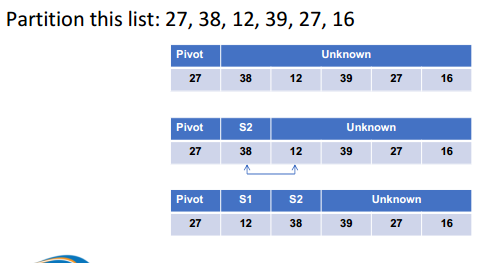
\includegraphics[scale=0.6]{Figures/sort_demo/quick_1.png}
    \caption{Partition technique}
    \label{fig:before_undo}
\end{minipage}\hfill
\begin{minipage}{0.45\textwidth}
    \centering
    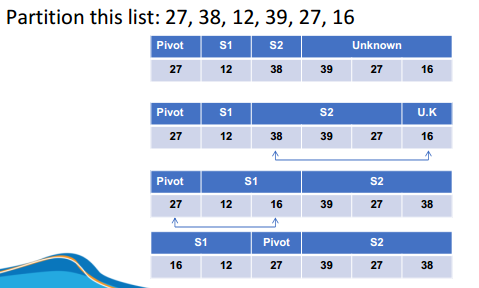
\includegraphics[scale=0.6]{Figures/sort_demo/quick_2.png}
    \caption{Partition technique}
    \label{fig:after_undo}
\end{minipage}
\end{figure}


\vspace{10pt}

\textbf{Another partition technique} ~\cite{ref7} 
\begin{figure}[h]
    \centering
    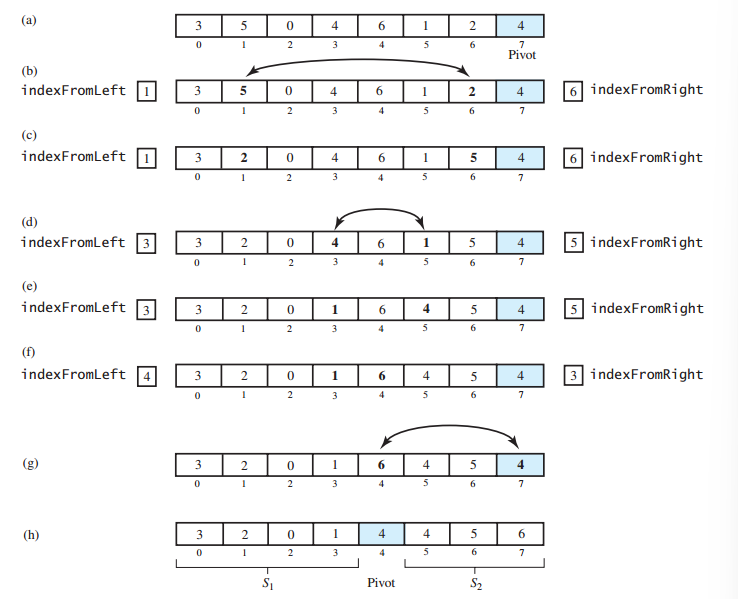
\includegraphics[width=0.55\textwidth]{Figures/sort_demo/quick_3.png}
    \caption{Partition technique 2}
    \label{fig:enter-label}
\end{figure}

\newpage

As the partition process is done recursively, it keeps on putting the pivot in its actual position in the sorted array. Repeatedly putting pivots in their actual position makes the array sorted.

\subsubsection{Complexity analysis}

\textbf{Time complexity:}
\begin{itemize}
    \item Best case: O(n log2n)  - occur when the pivot chosen at the each step divides the array into roughly equal halves, make balanced partitions, leading to efficient sorting.
    \item Average case: O(n log2n)
    \item Worst case: $O(n^2)$ - This rarely occurs when the pivot selection is poor, leading to unbalanced partitions (e.g., when the array is already sorted, and the first or last element is chosen as the pivot).
\end{itemize}

\textbf{Space complexity:} $O(1)$, if we don’t consider the recursive stack space. If we consider the recursive stack space then, in the worst case quicksort could make $O(n)$. ~\cite{ref10}

\subsubsection{Variants and optimizations}
\begin{itemize}[label=-]
    \item Median of three pivot selection: This pivot selection scheme assumes that the array has at least three entries. If you have only three entries, the pivot selection sorts them, so there is no need for the partition method or for a quick. ~\cite{ref7}
    \item Tail call optimization: partition function is in-place, but we need extra space for recursive function calls. Optimizing the recursive calls to minimize the depth of the recursive stack. By always sorting the smaller subarray first and using tail recursion for the larger subarray, the stack depth can be reduced.
\end{itemize}

\vspace{10pt}